\documentclass[12pt,letterpaper]{article}
\usepackage[utf8]{inputenc}
\usepackage[spanish]{babel}
\DeclareUnicodeCharacter{03B5}{\ensuremath{\varepsilon}}
\DeclareUnicodeCharacter{2192}{\ensuremath{\rightarrow}}
\usepackage[top=3.4cm,bottom=3cm,left=3cm,right=3.5cm,headheight=48pt,headsep=14pt]{geometry}
\usepackage{graphicx}
\usepackage{amsmath,amssymb}
\usepackage{booktabs}
\usepackage{float}
\usepackage{caption}
\captionsetup[table]{skip=8pt}
\captionsetup[lstlisting]{skip=4pt}
\usepackage{listings}
\usepackage{fancyhdr}
\usepackage{xcolor}
\usepackage{microtype}
\usepackage[hidelinks]{hyperref}

\graphicspath{{../img/}}

\pagestyle{fancy}
\fancyhf{}
\fancyhead[L]{\small\textit{\nouppercase{\rightmark}}}
\fancyhead[R]{\raisebox{-3pt}{
\includegraphics[height=1.45cm]{escudo_usa.png}}\hspace*{-1.2cm}}
\fancyfoot[C]{\thepage}
\renewcommand{\headrulewidth}{0.5pt}
\fancypagestyle{plain}{\fancyhf{}\fancyfoot[C]{\thepage}\renewcommand{\headrulewidth}{0pt}}

\lstset{
  basicstyle=\ttfamily\small,
  columns=fullflexible,
  keepspaces=true,
  showstringspaces=false,
  breaklines=true,
  xleftmargin=2em,
  aboveskip=0.8em,
  belowskip=0.8em,
  captionpos=t,
  extendedchars=true,
  literate={á}{{\'a}}1 {é}{{\'e}}1 {í}{{\'i}}1 {ó}{{\'o}}1 {ú}{{\'u}}1
           {ñ}{{\~n}}1 {Á}{{\'A}}1 {É}{{\'E}}1 {Í}{{\'I}}1 {Ó}{{\'O}}1
           {Ú}{{\'U}}1 {Ñ}{{\~N}}1 {ü}{{\"u}}1 {¿}{{?`}}1 {¡}{{!`}}1
           {ε}{{$\varepsilon$}}1 {→}{{$\rightarrow$}}1
}

\setlength{\parskip}{0.45em}
\setlength{\parindent}{0pt}
\setlength{\emergencystretch}{3em}

\newcommand{\tk}[1]{\texttt{#1}}
\newcommand{\nt}[1]{\textit{#1}}
\newcommand{\prim}{\textup{PRIMEROS}}
\newcommand{\sig}{\textup{SIGUIENTES}}
\newcommand{\pred}{\textup{PRED}}

\begin{document}

% ------------------------------------------------------------------ portada
\thispagestyle{plain}
\begin{center}
\vspace*{0.2cm}

\includegraphics[width=0.44\textwidth]{escudo_usa.png}\par
\vspace{2.4cm}
{\LARGE Diseño e implementación\\[4pt] de una gramática LL(1)\par}
\vspace{0.5cm}
{\large Un lenguaje con operaciones aritméticas, funciones\\ trigonométricas y asignación de variables\par}
\vspace{3.0cm}
{\large\bfseries Lenguajes de programación y traducción\par}
\vspace{0.9cm}
{\bfseries David Andrés Castellanos Angulo\par}
\vspace{2.7cm}
{\itshape Universidad Sergio Arboleda\\
Escuela de ciencias exactas e ingeniería\\
Bogotá D.C., 28 de septiembre de 2026\par}
\end{center}
\newpage

% ------------------------------------------------------------------ 1
\section{Objetivo del trabajo}

El trabajo pide diseñar e implementar una gramática LL(1) para un lenguaje de programación que soporte \tk{+}, \tk{-}, \tk{*}, \tk{/}, \tk{\%} y el valor absoluto, las funciones \tk{sin}, \tk{cos} y \tk{tan}, y la asignación de variables. Hay que garantizar las tres fases de análisis, mostrar los conjuntos PRIMEROS, SIGUIENTES y de predicción, y hacer pruebas de implementación.

\begin{figure}[H]
\centering
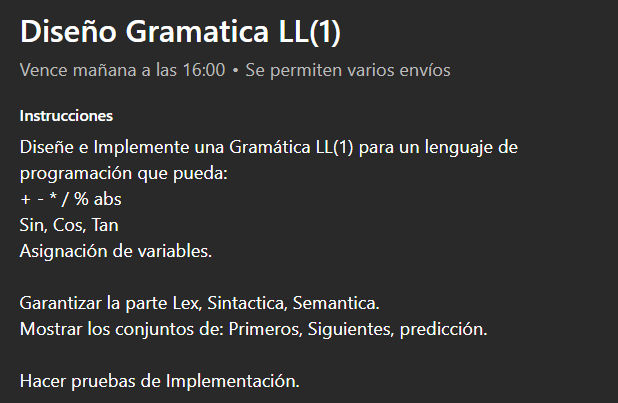
\includegraphics[width=0.72\textwidth]{enunciado.png}
\caption{Enunciado del trabajo.}
\end{figure}

Lo hice en Python, sin librerías externas, siguiendo el orden que vimos en clase para construir un analizador descendente recursivo: primero la gramática, después los conjuntos, después la verificación LL(1) y solo al final el código.

% ------------------------------------------------------------------ 2
\section{De la gramática natural a la gramática LL(1)}

No empecé escribiendo la gramática definitiva. La escribí como se lee en matemáticas y después le apliqué las transformaciones, que es donde está el trabajo de verdad.

\subsection{Primer borrador: recursión izquierda}

\noindent\begin{minipage}{\linewidth}
\begin{lstlisting}[caption={\texttt{grammars/borrador1\_recursion.txt}: la versión natural.}]
# Primer borrador: escribí la gramática como se lee en matemáticas.
# Tiene recursión izquierda en expr y en term, así que NO sirve para un ASDR.

prog     -> sents
sents    -> sent sents | ε
sent     -> ID asig expr fin

expr     -> expr mas term | expr menos term | term
term     -> term por fact | term entre fact | term modulo fact | fact

fact     -> menos fact | unidad
unidad   -> NUM | ID | abre expr cierra | barra expr barra | func abre expr cierra
func     -> abs | sin | cos | tan
\end{lstlisting}
\end{minipage}

La regla \nt{expr} $\rightarrow$ \nt{expr} \tk{+} \nt{term} dice exactamente lo que uno quiere: una suma es una suma seguida de un término. El problema es que tiene \textbf{recursión izquierda}, y eso rompe el descenso recursivo: la función \tk{expr()} se llamaría a sí misma como primera acción, sin haber consumido ningún token, y quedaría en un ciclo infinito.

Se ve también en los conjuntos. Le pasé este borrador al programa y reporta el conflicto:

\begin{lstlisting}
¿ES LL(1)? NO. Reglas con predicción en común:
  expr: reglas 5 y 6 comparten { ID, menos, NUM, abre, barra, abs, sin, cos, tan }
  expr: reglas 5 y 7 comparten { ID, menos, NUM, abre, barra, abs, sin, cos, tan }
  expr: reglas 6 y 7 comparten { ID, menos, NUM, abre, barra, abs, sin, cos, tan }
  term: reglas 8 y 9 comparten { ID, menos, NUM, abre, barra, abs, sin, cos, tan }
\end{lstlisting}

Las tres reglas de \nt{expr} predicen los mismos tokens, así que con un token de anticipación no hay forma de escoger.

\subsection{Segundo borrador: prefijo común}

Lo primero que intenté fue pasar la recursión al otro lado:

\begin{lstlisting}
expr -> term mas expr | term menos expr | term
\end{lstlisting}

Ya no hay recursión izquierda, pero aparece el otro obstáculo: las tres alternativas empiezan por \nt{term}, o sea, tienen \textbf{prefijo común}. El analizador tendría que consumir todo un término antes de saber cuál regla escogió, y eso es justamente lo que no se puede hacer con un solo token. El programa vuelve a reportar conflicto en \nt{expr} y en \nt{term} (\tk{grammars/borrador2\_prefijo.txt}).

\subsection{Las dos transformaciones}

La regla general para quitar la recursión izquierda inmediata es:
\[
A \rightarrow A\alpha \mid \beta \quad \Longrightarrow \quad A \rightarrow \beta A', \qquad A' \rightarrow \alpha A' \mid \varepsilon
\]

Aplicada a \nt{expr}, con $\alpha_1 =$ \tk{+} \nt{term}, $\alpha_2 =$ \tk{-} \nt{term} y $\beta =$ \nt{term}:
\[
\nt{expr} \rightarrow \nt{term}\ \nt{expr'}, \qquad
\nt{expr'} \rightarrow \tk{+}\ \nt{term}\ \nt{expr'} \mid \tk{-}\ \nt{term}\ \nt{expr'} \mid \varepsilon
\]

Y lo mismo en \nt{term} con \tk{*}, \tk{/} y \tk{\%}. La otra transformación, factorizar por la izquierda,
\[
A \rightarrow \alpha\beta_1 \mid \alpha\beta_2 \quad \Longrightarrow \quad A \rightarrow \alpha A', \qquad A' \rightarrow \beta_1 \mid \beta_2
\]
lleva al mismo resultado si se parte del segundo borrador: se saca el \nt{term} común y lo que queda detrás pasa a un no terminal nuevo. Por eso los dos caminos terminan en la misma gramática.

En el archivo los llamé \tk{expr\_r} y \tk{term\_r}, porque el apóstrofo no es cómodo en nombres de archivo y de funciones; en el informe los escribo \nt{expr'} y \nt{term'}.

\subsection{Gramática final}

\noindent\begin{minipage}{\linewidth}
\begin{lstlisting}[caption={\texttt{grammars/lenguaje.txt}.}]
# Gramática LL(1) del lenguaje
# Los no terminales son los símbolos de la izquierda; el resto son terminales.
# Los terminales en MAYÚSCULA son clases de token que entrega el analizador léxico.

prog     -> sents
sents    -> sent sents | ε
sent     -> ID asig expr fin

expr     -> term expr_r
expr_r   -> mas term expr_r | menos term expr_r | ε

term     -> fact term_r
term_r   -> por fact term_r | entre fact term_r | modulo fact term_r | ε

fact     -> menos fact | unidad

unidad   -> NUM
unidad   -> ID
unidad   -> abre expr cierra
unidad   -> barra expr barra
unidad   -> func abre expr cierra

func     -> abs | sin | cos | tan
\end{lstlisting}
\end{minipage}

Los terminales no son los símbolos sueltos sino \textbf{clases de token}: \tk{ID} para cualquier nombre de variable y \tk{NUM} para cualquier número, porque la gramática no puede enumerarlos uno por uno.

Tres cosas quedaron resueltas de una vez:

\begin{itemize}
  \item \textbf{Precedencia.} \nt{expr} agrupa sumas y restas, \nt{term} agrupa producto, división y módulo, y \nt{fact} queda más abajo. Como lo que está más abajo queda más profundo en el árbol, se evalúa primero: \tk{2 + 3 * 4} da 14.
  \item \textbf{Nada de recursión izquierda}, por la transformación anterior.
  \item \textbf{Nada de prefijos comunes.} Las cinco alternativas de \nt{unidad} empiezan cada una con un token distinto, y agrupé las cuatro funciones en \nt{func} para que \nt{unidad} tenga una sola alternativa que empiece por función.
\end{itemize}

% ------------------------------------------------------------------ 3
\section{Conjuntos y verificación LL(1)}

Como las transformaciones cambian la gramática, los conjuntos hay que \textbf{recalcularlos} sobre la versión final: el hecho de haber quitado la recursión izquierda no garantiza por sí solo que la gramática sea LL(1). Los calcula \tk{conjuntos.py}, el mismo programa del taller anterior, con algoritmos de punto fijo.

Para cada regla, la predicción se obtiene así:
{\small
\[
\pred(A \rightarrow \alpha) = \big(\prim(\alpha) - \{\varepsilon\}\big) \cup
\begin{cases}
\sig(A), & \text{si } \varepsilon \in \prim(\alpha),\\
\varnothing, & \text{si no.}
\end{cases}
\]}

\begin{table}[H]
\centering
\caption{PRIMEROS y SIGUIENTES de la gramática final.}
\footnotesize
\begin{tabular}{l p{5.0cm} p{5.4cm}}
\toprule
No terminal & PRIMEROS & SIGUIENTES \\
\midrule
\textit{prog} & \{\texttt{ID}, $\varepsilon$\} & \{\texttt{\$}\} \\
\textit{sents} & \{\texttt{ID}, $\varepsilon$\} & \{\texttt{\$}\} \\
\textit{sent} & \{\texttt{ID}\} & \{\texttt{ID}, \texttt{\$}\} \\
\textit{expr} & \{\texttt{ID}, \texttt{menos}, \texttt{NUM}, \texttt{abre}, \texttt{barra}, \texttt{abs}, \texttt{sin}, \texttt{cos}, \texttt{tan}\} & \{\texttt{fin}, \texttt{cierra}, \texttt{barra}\} \\
\textit{expr\_r} & \{\texttt{mas}, \texttt{menos}, $\varepsilon$\} & \{\texttt{fin}, \texttt{cierra}, \texttt{barra}\} \\
\textit{term} & \{\texttt{ID}, \texttt{menos}, \texttt{NUM}, \texttt{abre}, \texttt{barra}, \texttt{abs}, \texttt{sin}, \texttt{cos}, \texttt{tan}\} & \{\texttt{fin}, \texttt{mas}, \texttt{menos}, \texttt{cierra}, \texttt{barra}\} \\
\textit{term\_r} & \{\texttt{por}, \texttt{entre}, \texttt{modulo}, $\varepsilon$\} & \{\texttt{fin}, \texttt{mas}, \texttt{menos}, \texttt{cierra}, \texttt{barra}\} \\
\textit{fact} & \{\texttt{ID}, \texttt{menos}, \texttt{NUM}, \texttt{abre}, \texttt{barra}, \texttt{abs}, \texttt{sin}, \texttt{cos}, \texttt{tan}\} & \{\texttt{fin}, \texttt{mas}, \texttt{menos}, \texttt{por}, \texttt{entre}, \texttt{modulo}, \texttt{cierra}, \texttt{barra}\} \\
\textit{unidad} & \{\texttt{ID}, \texttt{NUM}, \texttt{abre}, \texttt{barra}, \texttt{abs}, \texttt{sin}, \texttt{cos}, \texttt{tan}\} & \{\texttt{fin}, \texttt{mas}, \texttt{menos}, \texttt{por}, \texttt{entre}, \texttt{modulo}, \texttt{cierra}, \texttt{barra}\} \\
\textit{func} & \{\texttt{abs}, \texttt{sin}, \texttt{cos}, \texttt{tan}\} & \{\texttt{abre}\} \\
\bottomrule
\end{tabular}
\end{table}

\begin{table}[H]
\centering
\caption{Conjuntos de predicción de las 24 reglas.}
\footnotesize
\begin{tabular}{r l p{6.0cm}}
\toprule
\# & Regla & PREDICCIÓN \\
\midrule
1 & \textit{prog} $\rightarrow$ \textit{sents} & \{\texttt{ID}, \texttt{\$}\} \\
2 & \textit{sents} $\rightarrow$ \textit{sent} \textit{sents} & \{\texttt{ID}\} \\
3 & \textit{sents} $\rightarrow$ $\varepsilon$ & \{\texttt{\$}\} \\
4 & \textit{sent} $\rightarrow$ \texttt{ID} \texttt{asig} \textit{expr} \texttt{fin} & \{\texttt{ID}\} \\
5 & \textit{expr} $\rightarrow$ \textit{term} \textit{expr\_r} & \{\texttt{ID}, \texttt{menos}, \texttt{NUM}, \texttt{abre}, \texttt{barra}, \texttt{abs}, \texttt{sin}, \texttt{cos}, \texttt{tan}\} \\
6 & \textit{expr\_r} $\rightarrow$ \texttt{mas} \textit{term} \textit{expr\_r} & \{\texttt{mas}\} \\
7 & \textit{expr\_r} $\rightarrow$ \texttt{menos} \textit{term} \textit{expr\_r} & \{\texttt{menos}\} \\
8 & \textit{expr\_r} $\rightarrow$ $\varepsilon$ & \{\texttt{fin}, \texttt{cierra}, \texttt{barra}\} \\
9 & \textit{term} $\rightarrow$ \textit{fact} \textit{term\_r} & \{\texttt{ID}, \texttt{menos}, \texttt{NUM}, \texttt{abre}, \texttt{barra}, \texttt{abs}, \texttt{sin}, \texttt{cos}, \texttt{tan}\} \\
10 & \textit{term\_r} $\rightarrow$ \texttt{por} \textit{fact} \textit{term\_r} & \{\texttt{por}\} \\
11 & \textit{term\_r} $\rightarrow$ \texttt{entre} \textit{fact} \textit{term\_r} & \{\texttt{entre}\} \\
12 & \textit{term\_r} $\rightarrow$ \texttt{modulo} \textit{fact} \textit{term\_r} & \{\texttt{modulo}\} \\
13 & \textit{term\_r} $\rightarrow$ $\varepsilon$ & \{\texttt{fin}, \texttt{mas}, \texttt{menos}, \texttt{cierra}, \texttt{barra}\} \\
14 & \textit{fact} $\rightarrow$ \texttt{menos} \textit{fact} & \{\texttt{menos}\} \\
15 & \textit{fact} $\rightarrow$ \textit{unidad} & \{\texttt{ID}, \texttt{NUM}, \texttt{abre}, \texttt{barra}, \texttt{abs}, \texttt{sin}, \texttt{cos}, \texttt{tan}\} \\
16 & \textit{unidad} $\rightarrow$ \texttt{NUM} & \{\texttt{NUM}\} \\
17 & \textit{unidad} $\rightarrow$ \texttt{ID} & \{\texttt{ID}\} \\
18 & \textit{unidad} $\rightarrow$ \texttt{abre} \textit{expr} \texttt{cierra} & \{\texttt{abre}\} \\
19 & \textit{unidad} $\rightarrow$ \texttt{barra} \textit{expr} \texttt{barra} & \{\texttt{barra}\} \\
20 & \textit{unidad} $\rightarrow$ \textit{func} \texttt{abre} \textit{expr} \texttt{cierra} & \{\texttt{abs}, \texttt{sin}, \texttt{cos}, \texttt{tan}\} \\
21 & \textit{func} $\rightarrow$ \texttt{abs} & \{\texttt{abs}\} \\
22 & \textit{func} $\rightarrow$ \texttt{sin} & \{\texttt{sin}\} \\
23 & \textit{func} $\rightarrow$ \texttt{cos} & \{\texttt{cos}\} \\
24 & \textit{func} $\rightarrow$ \texttt{tan} & \{\texttt{tan}\} \\
\bottomrule
\end{tabular}
\end{table}

La condición LL(1) es que, para dos reglas distintas del mismo no terminal,
\[
\pred(A \rightarrow \alpha) \cap \pred(A \rightarrow \beta) = \varnothing .
\]

El programa compara los pares regla por regla y confirma que se cumple:

\begin{lstlisting}
¿ES LL(1)? SÍ: las reglas de cada no terminal tienen predicciones disjuntas.
\end{lstlisting}

\begin{figure}[H]
\centering
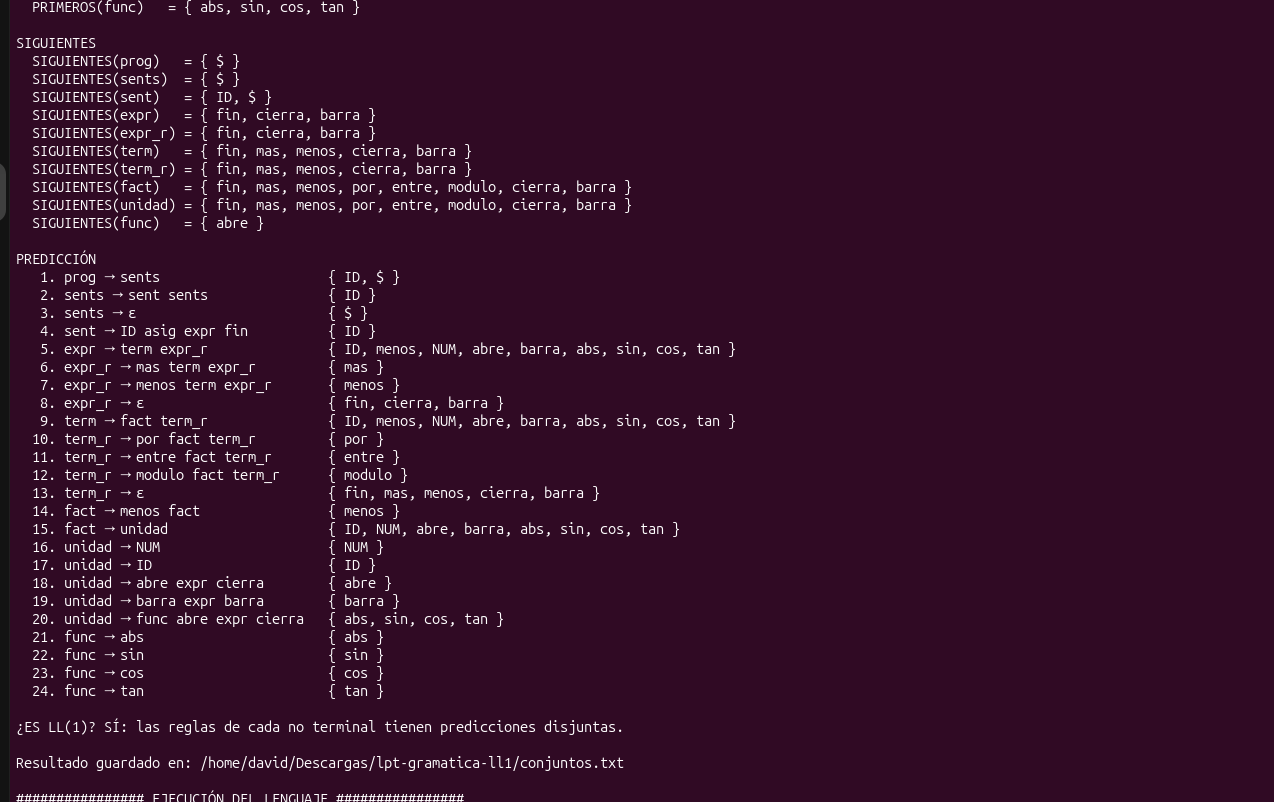
\includegraphics[width=0.92\textwidth]{evid_conjuntos.png}
\caption{Conjuntos SIGUIENTES y de predicción de la gramática final, con la verificación LL(1).}
\end{figure}

Se puede revisar a simple vista en la tabla: las tres reglas de \nt{expr'} predicen \tk{mas}, \tk{menos} y \{\tk{fin}, \tk{cierra}, \tk{barra}\}; y las cinco de \nt{unidad} predicen cada una un token distinto. El caso de \nt{expr'} $\rightarrow \varepsilon$ es el que usa SIGUIENTES: como la regla puede desaparecer, se predice con los tokens que pueden venir después.

Vale la pena aclarar algo que vimos en clase: un conflicto LL(1) no significa que la gramática sea ambigua. Los dos borradores de la sección anterior generan el mismo lenguaje que la versión final y no son ambiguos; simplemente no se pueden analizar con un solo token de anticipación. LL(1) implica que no hay ambigüedad, pero al revés no.

% ------------------------------------------------------------------ 4
\section{Construcción del analizador}

Seguí los cinco pasos del ASDR: definir la gramática y su símbolo inicial, calcular PRIMEROS, SIGUIENTES y predicción, verificar que las predicciones sean disjuntas, escribir una función por no terminal con una operación \tk{emparejar} para los terminales, y finalmente tomar el primer token, llamar al símbolo inicial y comprobar el fin de entrada.

\subsection{Análisis léxico}

\tk{lexico.py} recorre el texto y arma la lista de tokens. Reconoce enteros y reales, identificadores, las palabras reservadas, los símbolos y los comentarios con \tk{\#}. Cada token guarda su línea y columna, que es lo que permite reportar los errores con la posición exacta:

\begin{lstlisting}
Error léxico: línea 2, columna 7: símbolo no reconocido '@'.
\end{lstlisting}

Al final agrega el token \tk{\$}, que es el marcador de fin de entrada que aparece en los conjuntos SIGUIENTES.

\subsection{Análisis sintáctico: una función por no terminal}

Cada regla de la gramática se volvió una función, y cada alternativa se decide con su conjunto de predicción. Este es \nt{fact}, que tiene dos alternativas:

\noindent\begin{minipage}{\linewidth}
\begin{lstlisting}[language=Python,basicstyle=\ttfamily\footnotesize,caption={\texttt{fact -> menos fact | unidad} en \texttt{sintactico.py}.}]
def fact(self):
    if self.token.clase == "menos":        # PRED = { - }
        signo = self.emparejar("menos")
        return ("neg", self.fact(), signo.linea)
    if self.token.clase in PRED_UNIDAD:    # PRED = PRIMEROS(unidad)
        return self.unidad()
    self.error_sintaxis("un número, una variable, '(', '|' o una función")
\end{lstlisting}
\end{minipage}

Los terminales se consumen con \tk{emparejar}, que es la única función que avanza sobre la entrada:

\noindent\begin{minipage}{\linewidth}
\begin{lstlisting}[language=Python,basicstyle=\ttfamily\footnotesize]
def emparejar(self, esperado):
    if self.token.clase != esperado:
        self.error_sintaxis(NOMBRES.get(esperado, esperado))
    actual = self.token
    self.pos += 1
    return actual
\end{lstlisting}
\end{minipage}

Y el análisis termina comprobando que no sobre nada: si después de la última sentencia todavía hay tokens, es error, aunque todo lo anterior estuviera bien.

\subsection{Asociatividad: el acumulador}

Aquí está el detalle que más cuidado pide. Al quitar la recursión izquierda, la gramática quedó repitiendo por la derecha, pero la resta no es asociativa por la derecha:
\[
\underbrace{(4 - 5) - 10}_{-11} \;\neq\; \underbrace{4 - (5 - 10)}_{9}
\]

La transformación de la gramática no decide cómo evaluar: eso lo deciden las acciones semánticas. Por eso \nt{expr'} recibe un acumulador con lo que ya se construyó a la izquierda y lo va envolviendo en cada vuelta:

\noindent\begin{minipage}{\linewidth}
\begin{lstlisting}[language=Python,basicstyle=\ttfamily\footnotesize]
def expr_r(self, acc):
    if self.token.clase in PRED_EXPR_R:    # PRED = { +, - }
        operador = self.token
        self.emparejar(operador.clase)
        derecha = self.term()
        nuevo = ("bin", OPERADORES[operador.clase], acc, derecha, operador.linea)
        return self.expr_r(nuevo)
    return acc                             # expr' -> epsilon
\end{lstlisting}
\end{minipage}

Con \tk{4 - 5 - 10} el acumulador pasa por \tk{4}, luego \tk{(4 - 5)} y luego \tk{((4 - 5) - 10)}, que da $-11$. Hay una prueba automática exactamente para eso.

\subsection{Traza del análisis}

Para poder revisar las decisiones agregué la opción \tk{--traza}, que muestra qué regla se aplicó en cada paso y qué quedaba por leer:

\noindent\begin{minipage}{\linewidth}
\begin{lstlisting}[basicstyle=\ttfamily\scriptsize,caption={Traza de \texttt{resta = 4 - 5 - 10;}, con la opción \texttt{--traza}.}]
Paso  Función / acción           Entrada pendiente
1     prog -> sents              resta = 4 - 5 - 10 ; $
2     sents -> sent sents        resta = 4 - 5 - 10 ; $
3     sent -> ID = expr ;        resta = 4 - 5 - 10 ; $
4     emparejar resta            = 4 - 5 - 10 ; $
5     emparejar =                4 - 5 - 10 ; $
6     expr -> term expr'         4 - 5 - 10 ; $
7     term -> fact term'         4 - 5 - 10 ; $
8     fact -> unidad             4 - 5 - 10 ; $
9     unidad -> NUM              4 - 5 - 10 ; $
10    emparejar 4                - 5 - 10 ; $
11    term' -> ε                 - 5 - 10 ; $
12    expr' -> - term expr'      - 5 - 10 ; $
13    emparejar -                5 - 10 ; $
14    term -> fact term'         5 - 10 ; $
15    fact -> unidad             5 - 10 ; $
16    unidad -> NUM              5 - 10 ; $
17    emparejar 5                - 10 ; $
18    term' -> ε                 - 10 ; $
19    expr' -> - term expr'      - 10 ; $
20    emparejar -                10 ; $
21    term -> fact term'         10 ; $
22    fact -> unidad             10 ; $
23    unidad -> NUM              10 ; $
24    emparejar 10               ; $
25    term' -> ε                 ; $
26    expr' -> ε                 ; $
27    emparejar ;                $
28    sents -> ε                 $
29    fin de entrada: aceptada   $
\end{lstlisting}
\end{minipage}

\begin{figure}[H]
\centering
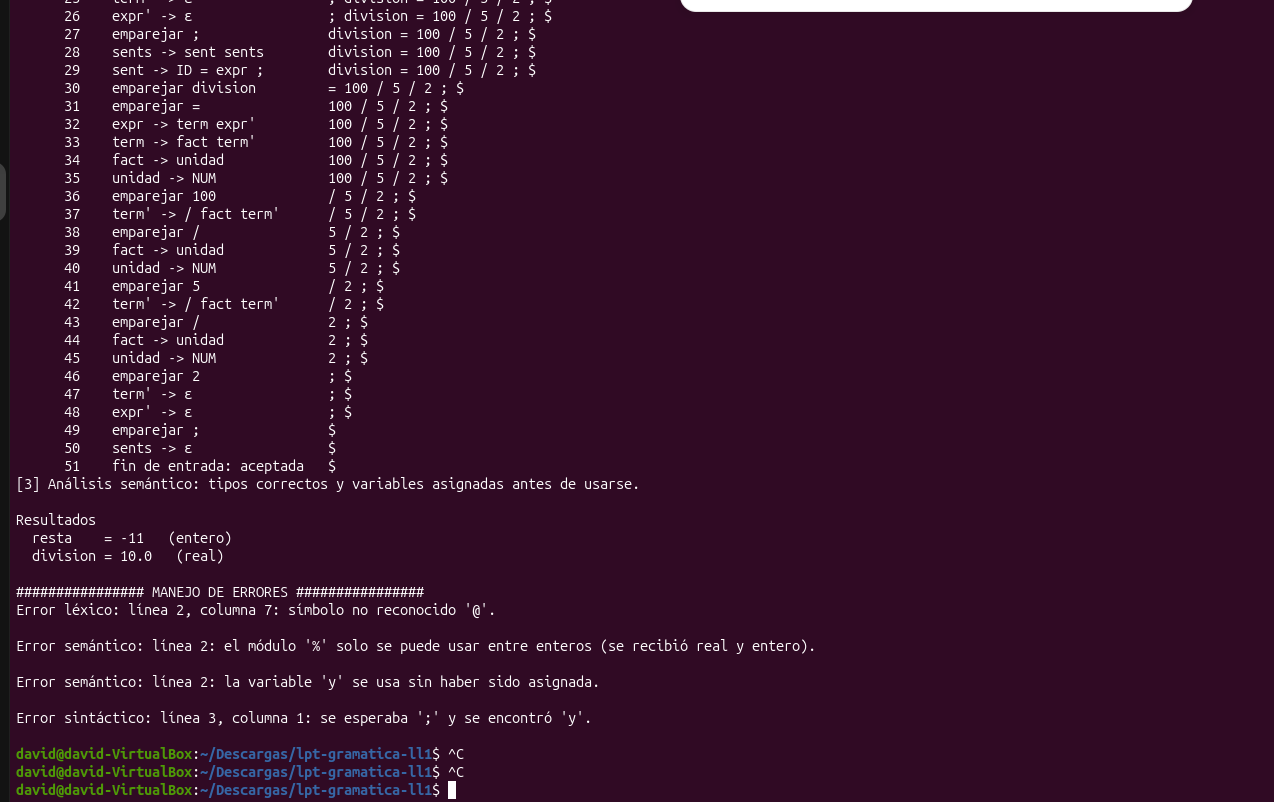
\includegraphics[width=0.92\textwidth]{evid_traza.png}
\caption{Final de la traza, aceptación de la entrada y los cuatro errores de las tres fases.}
\end{figure}

Se ve el patrón del descenso recursivo: baja hasta \nt{unidad} para tomar el \tk{4}, sube cerrando \nt{term'} con $\varepsilon$, y solo entonces \nt{expr'} toma el primer \tk{-}. Al final la entrada queda en \tk{\$} y se acepta.

\subsection{Análisis semántico}

La gramática dice qué está bien formado, no qué tiene sentido. \tk{x = y + 1;} es sintácticamente perfecto aunque \tk{y} no exista, y no hay forma de expresar eso en una gramática libre de contexto. Por eso \tk{semantico.py} recorre el árbol con una tabla de símbolos y revisa:

\begin{itemize}
  \item que una variable esté asignada antes de usarse;
  \item los tipos: \tk{+}, \tk{-} y \tk{*} dan entero solo si los dos operandos son enteros; \tk{/} siempre da real; \tk{\%} exige enteros de los dos lados; \tk{sin}, \tk{cos} y \tk{tan} devuelven real; \tk{abs} y \tk{|x|} conservan el tipo;
  \item que no se divida entre la constante cero.
\end{itemize}

\begin{lstlisting}
Error semántico: línea 2: la variable 'y' se usa sin haber sido asignada.
Error semántico: línea 2: el módulo '%' solo se puede usar entre enteros (se recibió real y entero).
\end{lstlisting}

Después, una segunda pasada evalúa el programa y llena la tabla con el valor de cada variable.

% ------------------------------------------------------------------ 5
\section{Pruebas de implementación}

En \tk{test\_implementacion.py} hay 36 pruebas automáticas con \tk{unittest}:

\begin{table}[H]
\centering
\caption{Grupos de pruebas.}
\small
\begin{tabular}{l r p{7.6cm}}
\toprule
Grupo & Pruebas & Qué revisa \\
\midrule
Léxico & 6 & tokens, comentarios, reales, símbolos inválidos \\
Sintáctico & 12 & precedencia, asociatividad, paréntesis, menos unario, traza, tokens sobrantes y errores \\
Semántico & 6 & tipos, variable sin asignar, módulo con reales, división por cero \\
Funciones & 3 & \tk{sin}, \tk{cos}, \tk{tan} y funciones anidadas \\
Gramática & 6 & LL(1), sin recursión izquierda, sin prefijos comunes, PRIMEROS, SIGUIENTES y predicción \\
Transformaciones & 2 & los dos borradores sí tienen conflictos \\
Ejemplos & 2 & los archivos de \tk{ejemplos/} dan el resultado y el error esperados \\
\bottomrule
\end{tabular}
\end{table}

\begin{figure}[H]
\centering
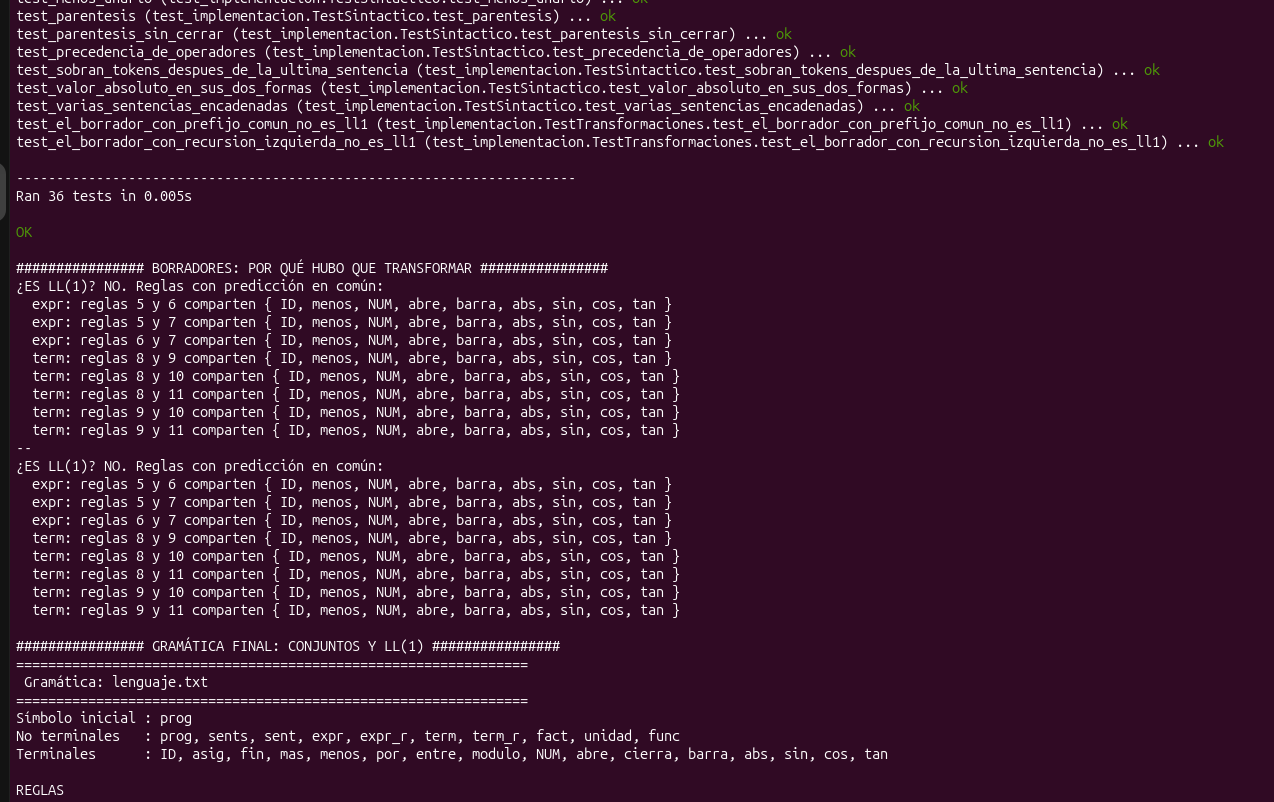
\includegraphics[width=0.92\textwidth]{evid_pruebas.png}
\caption{Las 36 pruebas y los conflictos que reportan los dos borradores.}
\end{figure}

Las dos pruebas de transformaciones son las que dejan constancia de por qué la gramática quedó así: comprueban que los borradores tienen conflicto en \nt{expr} y \nt{term}, y la de la gramática final comprueba que ya no lo tiene. Las de precedencia y asociatividad revisan el otro lado: que además de analizar, el resultado sea el correcto.

\begin{lstlisting}[caption={Comandos usados.}]
chmod +x run_all.sh
./run_all.sh                                 # pruebas, borradores, conjuntos y ejemplos
python3 main.py ejemplos/demo.lp             # análisis completo de un programa
python3 main.py ejemplos/demo.lp --traza     # traza del análisis
python3 main.py --conjuntos                  # PRIMEROS, SIGUIENTES, predicción y LL(1)
\end{lstlisting}

% ------------------------------------------------------------------ 6
\section{Ejemplo completo}

\noindent\begin{minipage}{\linewidth}
\begin{lstlisting}[caption={\texttt{ejemplos/demo.lp}.}]
# Programa de prueba del lenguaje

base = 12;
altura = 5;
area = base * altura / 2;

resto = 17 % base;
desfase = |3 - 10|;
negativo = -base + 4;

angulo = 0.7853981634;          # 45 grados en radianes
razon = sin(angulo) / cos(angulo);
mezcla = abs(-2.5) * (base + 1) - tan(0.0);
\end{lstlisting}
\end{minipage}

\noindent\begin{minipage}{\linewidth}
\begin{lstlisting}[caption={Salida de \texttt{python3 main.py ejemplos/demo.lp}.}]
[1] Análisis léxico: 72 tokens reconocidos.
[2] Análisis sintáctico: 9 sentencias, sin errores.
[3] Análisis semántico: tipos correctos y variables asignadas antes de usarse.

Resultados
  base     = 12   (entero)
  altura   = 5   (entero)
  area     = 30.0   (real)
  resto    = 5   (entero)
  desfase  = 7   (entero)
  negativo = -8   (entero)
  angulo   = 0.785398   (real)
  razon    = 1.0   (real)
  mezcla   = 32.5   (real)
\end{lstlisting}
\end{minipage}

\begin{figure}[H]
\centering
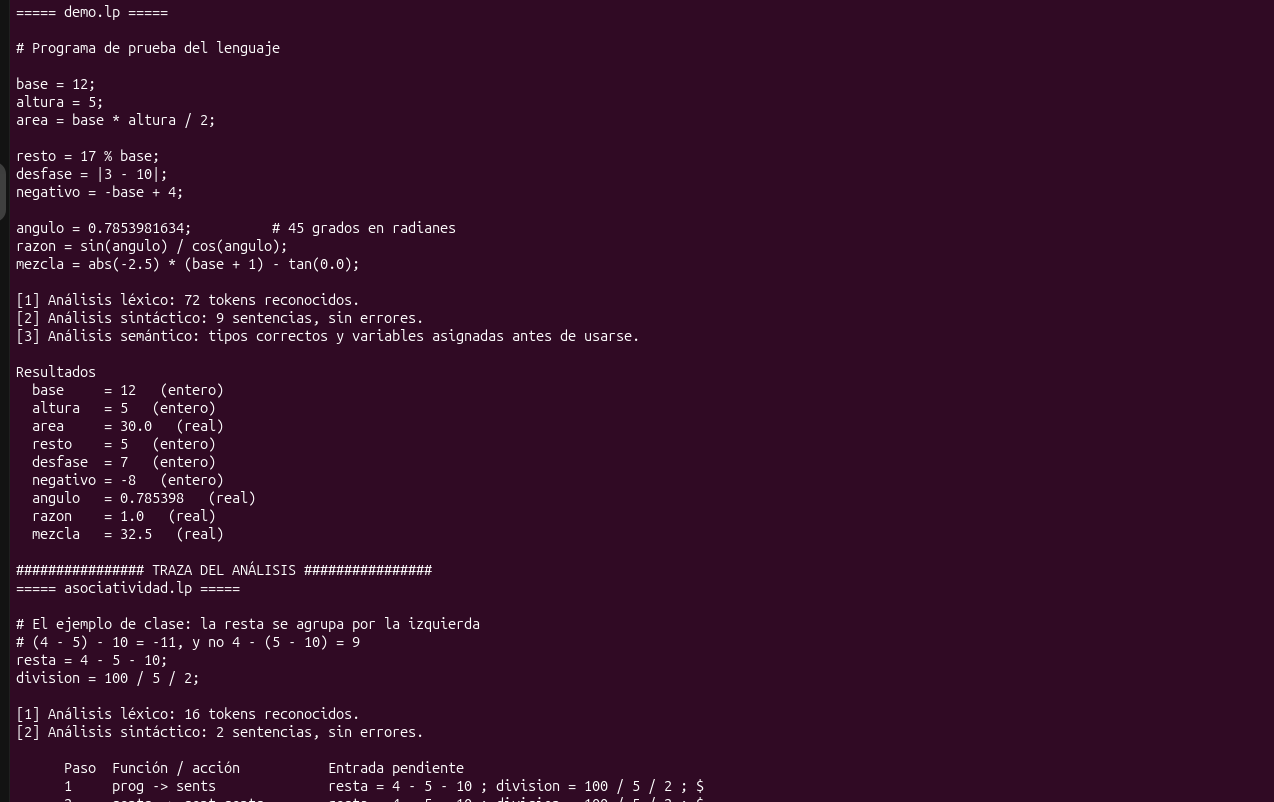
\includegraphics[width=0.92\textwidth]{evid_ejecucion.png}
\caption{Ejecución de \texttt{demo.lp} en Ubuntu.}
\end{figure}

Se puede comprobar a mano: \tk{area} es $12 \times 5 / 2 = 30$ y queda real porque hay una división; \tk{resto} es $17 \bmod 12 = 5$ y queda entero; \tk{desfase} es $|3-10| = 7$; y \tk{razon} es $\tan(45^\circ) = 1$, calculado como seno sobre coseno.

% ------------------------------------------------------------------ 7
\section{Conclusiones}

\begin{itemize}
  \item La gramática no quedó LL(1) de entrada. Quedó LL(1) después de aplicar las transformaciones sobre el borrador natural, y eso solo se puede afirmar recalculando los conjuntos de predicción sobre la versión final.
  \item Los conjuntos de predicción no son un ejercicio aparte: son literalmente las condiciones de los \tk{if} del analizador. Por eso el código no necesita retroceso.
  \item Quitar la recursión izquierda arregla el análisis pero no la evaluación. La asociatividad por la izquierda hay que devolverla con el acumulador, y sin eso \tk{4 - 5 - 10} daría 9 en vez de $-11$.
  \item Separar las tres fases deja cada error donde corresponde: un símbolo raro lo ve el léxico, un \tk{;} faltante lo ve el sintáctico y una variable sin asignar solo la puede ver el semántico.
\end{itemize}

\end{document}
